\documentclass{article}
\usepackage[utf8]{inputenc}
\usepackage{geometry}
%%\usepackage{multicol}
\usepackage{graphicx}
\usepackage{graphics}
\usepackage{amsmath}
\usepackage{hyperref}
\usepackage{amsmath}
\usepackage{svg}
\usepackage{amssymb}





	
\begin{document}
	\title{\textbf{Eigenvalues of updated matrix:\\
		 Symmetric row/column update}}
	\author{Viktor Kristensen Haldborg\\
		Student Nr: 201607139 \\
		AU ID: 540203}
	\date{\today}
	\maketitle	
%%\begin{multicols}{2}


		


\subsection*{Introduction}
I have been given the examination project (39 mod 22)=17 with the task of diagonalizing a matrix A given a matrix D and an update matrix W which gives rise to updated eigenvalues. 
\subsection*{Theory}
The matrix A to be diagonalized is given in the form
\begin{equation}
\mathbf{A}=\mathbf{D}+\mathbf{e}(p) \mathbf{u}^{T}+\mathbf{u e}(p)^{T}
\label{Aa}
\end{equation}
where $\mathbf{D}$ is a diagonal matrix with diagonal elements $\left\{d_{i} | i=1, \ldots, n\right\}, \mathbf{e}(p)$ is the unit vector in the $p$ -direction, and $\mathbf{u}$ is a given update vector where the $p$ -th element can be assumed to equal zero, $u_{p}=0,$ without loss of generality. Expressing the eigenvalue equation in terms of equation (\ref{Aa}) and subtracting $\lambda \mathbf{A}$ yields:
\begin{equation}
0=(\mathbf{D}-\lambda) \mathbf{x}+\mathbf{e}(p) \mathbf{u}^{T} \mathbf{x}+\mathbf{u e}(p)^{T} \mathbf{x}
\end{equation}
We are ai priori given that $u_{p}=0$, so for $k=p$ we get:
\begin{equation}
0=\left(d_{p}-\lambda\right) x_{p}+\sum_{k=1}^{n}u_{k}x_{k}
\label{subs}
\end{equation}
and for $k \neq p$ we get:
\begin{equation}
0=\left(d_{k}-\lambda\right) x_{k}+u_{k} x_{p}
\label{omskriv}
\end{equation}
By summation of all the elements from $k=1$ to $n$, equation ($\ref{omskriv}$) can be expressed as:
\begin{equation}
0=\sum_{k=1}^{n}u_{k}x_{k}+\sum_{k\neq p}^{n}\frac{u_{k}^{2} x_{p}}{\left(d_{k}-\lambda\right)}
\label{omskriv1}
\end{equation}
Substitution of equation ($\ref{subs}$) gives the secular equation written in the form: 
\begin{equation}
0=-\left(d_{p}-\lambda\right)+\sum_{k \neq p}^{n}\frac{u_{k}^{2}}{\left(d_{k}-\lambda\right)}=P_{A}
\label{poly}
\end{equation}
Solutions to this equation will yield the updated eigenvalues.
The secular equation (\ref{poly}) is ill defined for $\lambda=d_{k} \forall k\neq p$.

The polynomial will not be differentiable on all $\mathbb{R}$, however it will be piece-wise differentiable in between the singularities:

\begin{equation}
1+\sum_{k \neq p}^{n}\frac{u_{k}^{2}}{{\left(d_{k}-\lambda\right)}^{2}}
\label{omskriv}
\end{equation}
Which yields a strictly positive function defined on the same domain as equation (\ref{poly}).

By pulling out the n'th term in the sum of (\ref{poly}) and multiplying by $\lambda-d_{n}$;
\begin{equation}
0=u_{n}^{2}+(d_{n}-\lambda)\left[-\left(d_{p}-\lambda\right)+\sum_{k \neq p}^{n-1}\frac{u_{k}^{2}}{\left(d_{k}-\lambda\right)}\right]
\label{pullingout}
\end{equation}
it becomes evident, by the factoring of $\left(d_{n}-\lambda\right)$, that $\lambda=d_{n}$ will be a root of this polynomial if $u_{n}=0$. However by default, a computer would zero out the term without any subsequent notion of its domain. To circumvent this it is clear that by multiplication;
\begin{equation}
\left(\prod_{k\neq p}^{n} (d_{k}-\lambda)\right)\left[-\left(d_{p}-\lambda\right)+\sum_{k \neq p}^{n}\frac{u_{k}^{2}}{\left(d_{k}-\lambda\right)}\right]
\label{analyticalprod}
\end{equation}
equation (\ref{analyticalprod}) may be constructed and used by the computer to have a continuously defined polynomial to work on whilst still retaining all information about the eigenvalues in (\ref{poly}).


The differentiated expression is found by application of the product rule:

\begin{equation}
\left(\prod_{k \neq p}^{n} (d_{k}-\lambda)\right)\left(1+\sum_{k \neq p}^{n}\frac{u_{k}^{2}}{{\left(d_{k}-\lambda\right)}^{2}}-\left(\sum_{k \neq p}^{n}\frac{1}{\left(d_{k}-\lambda\right)}\right)P_{A}\right)
\label{derivprod}
\end{equation}


\subsection*{Numerical solutions}
To obtain the roots to (\ref{poly}) the method of root finding using the Newton Raphson method is implemented and built for multidimensional purposes. This is done under the assumption that no degeneracy is introduced by the update. The function used is the one obtained in (\ref{poly}) and the multidimensional Newton Raphson method has been coded using the analytical derivative found from the secular equation (\ref{omskriv}).
As such, an interval search can be brought to light since knowledge about the placement of the roots can be used to quickly generate an initial guess and break out of the given interval search when the root is obtained.
When $u_{k}=0$ for some $k$ different from $p$ the computer changes the function by zeroing out the $k'th$ term, and an addition to the code has thus been made to add in the missing eigenvalues which then must be exactly located outside the interval search, i.e on the given discontinuity $d_{k}$. If the trivial case is generated for which the update matrix is 0 all along the diagonal the main body of the code(interval search) will be skipped. A plethora of information for the specific implemenentations in A) and B) is given in the folders.
\newpage

For the scenario of diagonalizing a matrix A for which the update gives rise to degeneracy in the eigenvalues, a different method has been brought to use. The reexpression of the secular equation obtained in (\ref{analyticalprod}) along with its derivative (\ref*{derivprod}) has been implemented to search for the roots by "shooting" out initial guesses and then letting the Newton Raphson method converge to the roots. A sorting mechanism has then been implemented to sort the list of converged results. To find the degeneracy of a given root the function and its analytical derivative is used to find eigenvalues with degeneracy up to 3.
\begin{figure}[h]
	\centering
	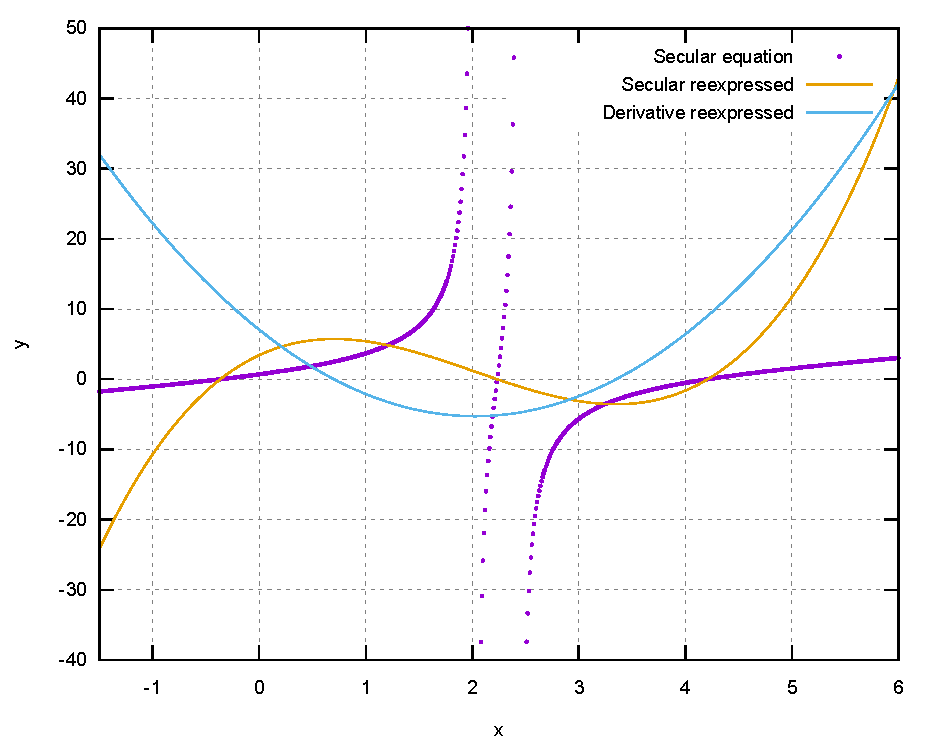
\includegraphics[width=0.9\linewidth]{Functions}
	\caption{Plot of the secular equation obtained in (\ref{poly}), the reexpressed form (\ref{analyticalprod}) along with its derivative (\ref{derivprod}) for n=3, no degeneracy and n-1 discontinuities.} 
	\label{fig:functions}
\end{figure}


The results are presented in .txt files for the A),B) and C) part and are compared with the diagonalization of the same matrix using the Jacobi sweeps.

\subsection*{Discussion}
Different opportunities were present, when trying to find the roots to the secular equation, such as bisection or simply brute forcing a solution by linearly running through the intervals and redefining the search based on if statements. However this would give rise to running through the listed elements more than once. Another way which could be achieved more easily was using binary search $O(log(n))$ since the intervals would be ordered by default when searching the original secular equation. However the high resolution needed in the listing of points and the fact that the points would have to be run through and listed beforehand makes it redundant even as a guessing tool if no list is given beforehand.
$\newline$
$\newline$
Using the re-expressed secular equation to form a general basis to find solutions to the original secular equations seems to be the best way to go about treating the problem numerically given the ill defined points in the original secular equation. However given the made assumptions in part A) and B) the technique searching the intervals proved to have much greater stability when scaled, and much less tweaking of parameters was required since it would be fairly easy to find an adequate guess to be within convergence radius of the Newton's method.




\begin{figure}[h]
	\begin{center}
		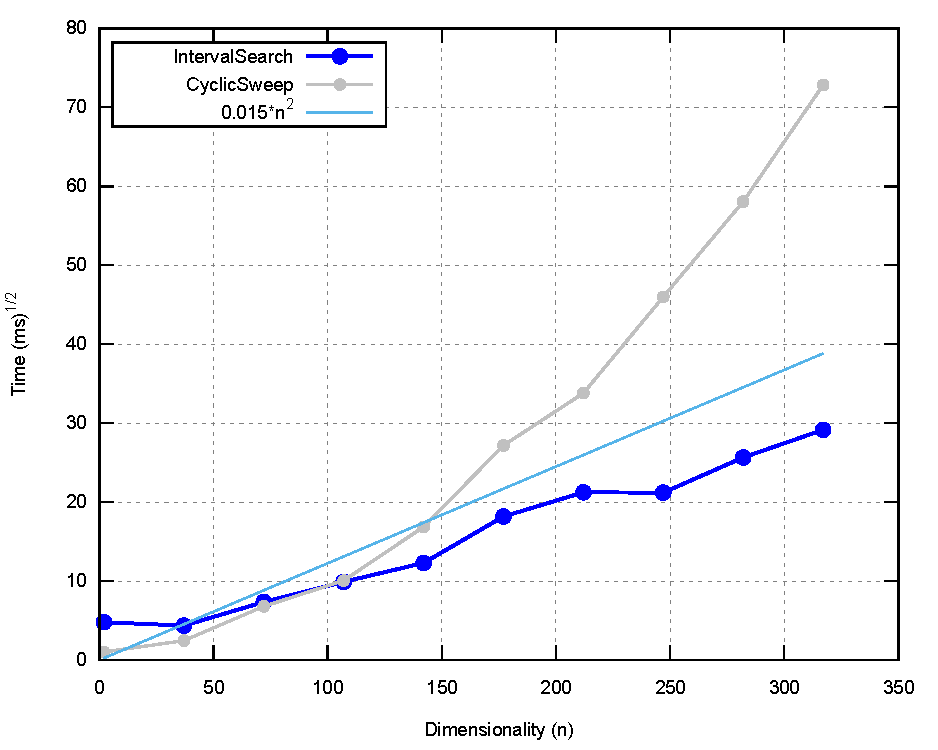
\includegraphics[width=0.8\linewidth]{TimeA}
		\caption{Plot of the operation time as a function of the dimensionality of the problem. It shows the operation time for the implemented interval search, for the assumptions made in part A), along with the diagonalization of the same matrices using Jacobian cyclic sweeps. Alongside it is a reference function $0.015*n^{2}$ for which the interval search seems to lie well within. The cyclic Jacobian seems to be faster for low dimensions and then takes off showing its $O(n^{3})$ dependancy.}
		\label{fig:timea}
	\end{center}
\end{figure}



\begin{figure}[h]
	\centering
	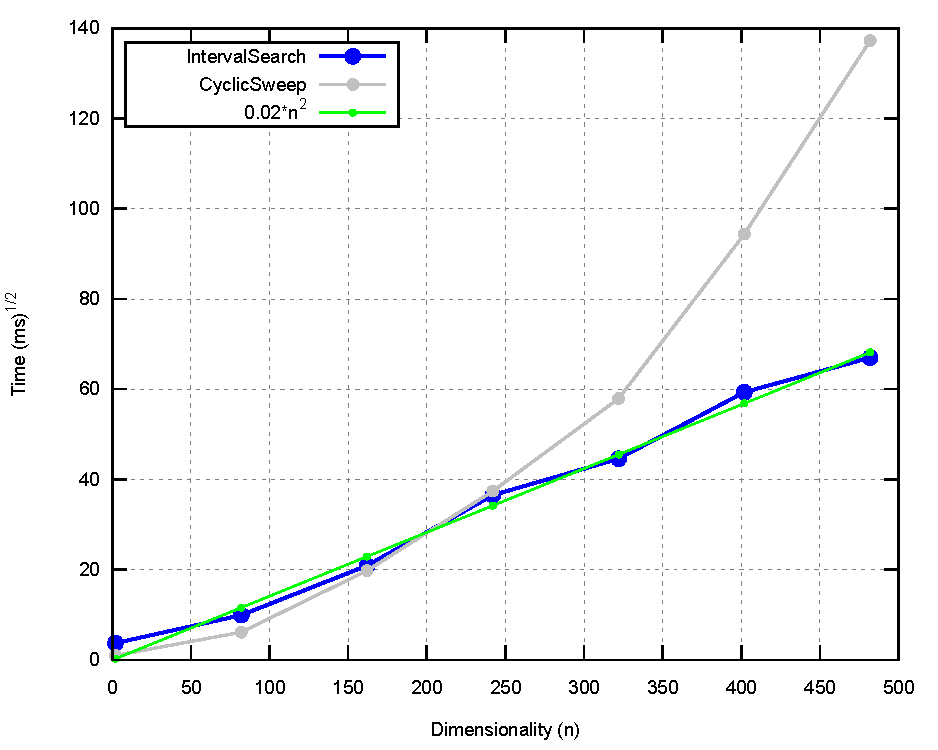
\includegraphics[width=0.8\linewidth]{TimeB}
	\caption{Plot of the operation time as a function of the dimensionality of the problem. It shows the operation time for the implemented interval search, for the assumptions made in part B), along with the diagonalization of the same matrices using Jacobian cyclic sweeps. Alongside it is a reference function $0.02*n^{2}$ for which the interval search seems follow in a linear fashion, as expected. An additional reorganization of the $u$ vector had to be done and therefore another search through $n$ elements was needed, which explains the higher operation time and $n$ dependance compared to the operation time displayed in figure (\ref{fig:timea}). }
	\label{fig:timeb}
\end{figure}


\newpage
\medskip

\begin{thebibliography}{9}
	\bibitem{latexcompanion} 
	Dimitri.V. Fedorov, ”Yet Another Introduction to Numerical Methods”, 2020.
	
\end{thebibliography}
\end{document}
